\subsection{IntAct curated physical interactions: do gated antigens co-complex?}
\label{sec:intact}
A biclonal AND gate assumes the two gated antigens can be engaged as
independent surface targets; if two antigens instead reside in a shared
membrane complex, cis-engagement could alter avidity, sterically couple the
two scFv binding events, or expose a single point of escape through loss of
the complex. We audited curated physical interactions from IntAct (EBI
PSICQUIC REST, MITAB 2.5) for all @NGENES@ genes in the study universe
(@NOK@ with a UniProt accession; the four pseudogene/unresolved cases carry
no record). For each gene we collected the PSICQUIC interaction count and
the full paginated MITAB record; evidence was restricted to human--human
pairs (taxid 9606 both sides) with a physical PSI-MI interaction type
(direct interaction, association, physical association, proximity), and
self-interactions were excluded from pairwise analysis.

\paragraph{Calibration gate.} Pre-registered gates PASSED: (G1) the ERBB2
partner set contains both canonical heterodimer partners EGFR and ERBB3
(observed @GATEONE@); (G2) for all 15 focus genes (7 antigens, 4 references,
4 intracellular controls) the paginated MITAB row count equals the
independent PSICQUIC count endpoint (observed @GATETWO@); (G3) all 4
intracellular controls return nonzero curated counts, confirming the
pipeline resolves non-surface proteins (observed @GATETHREE@).

\paragraph{Antigen-pair co-complex test.} @NEDGES@ of the 21 AND-gate
antigen pairs carry a curated human physical edge (@PAIRLIST@; fraction
@PAIRFRAC@). A permutation null over @NPERM@ random 7-gene background
subsets gives $p=@PUNIF@$; a degree-matched null matching each antigen to a
background gene within $\pm25\%$ curated degree (@NMATCHED@ valid draws)
gives $p=@PMATCH@$. @H1VERDICT@

\paragraph{Interaction degree: study-bias audit.} Median curated degree is
@MEDG@ (gated) versus @MEDB@ (background) (Mann--Whitney $p=@PMW@$);
any-record coverage is @COVG@ gated versus @COVB@ background (Fisher odds
ratio @COVOR@, $p=@COVP@$). Stratified by epitope topology class, the
degree contrast is @STRATSUM@. @H2VERDICT@

\paragraph{Per-antigen interaction context.} @ANTIGENBLOCK@

\begin{figure}[t]
\centering
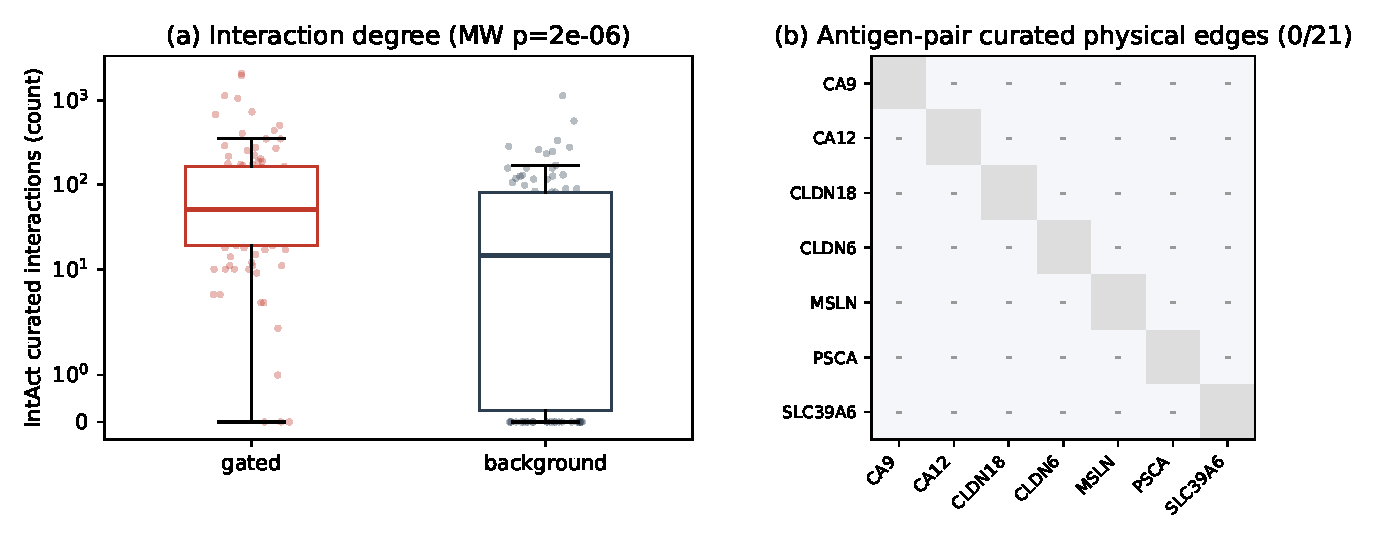
\includegraphics[width=\linewidth]{intact_fig.pdf}
\caption{IntAct curated interaction context. (a) Curated physical
interaction degree for gated versus background genes (symlog axis; boxes
show median and quartiles). (b) Pairwise curated physical edges among the
seven AND-gate antigens (Y = human physical curated edge in IntAct; grey
diagonal excluded).}
\label{fig:intact}
\end{figure}
